\documentclass[border=10pt]{standalone}
\usepackage{amsmath,amssymb}
\usepackage{tikz}
\usetikzlibrary{arrows.meta,positioning,backgrounds,fit}
\definecolor{srccol}{RGB}{37,99,235}
\definecolor{rxcol}{RGB}{5,150,105}
\definecolor{boxcol}{RGB}{241,245,249}
\newcommand{\herm}{^{H}}
\begin{document}
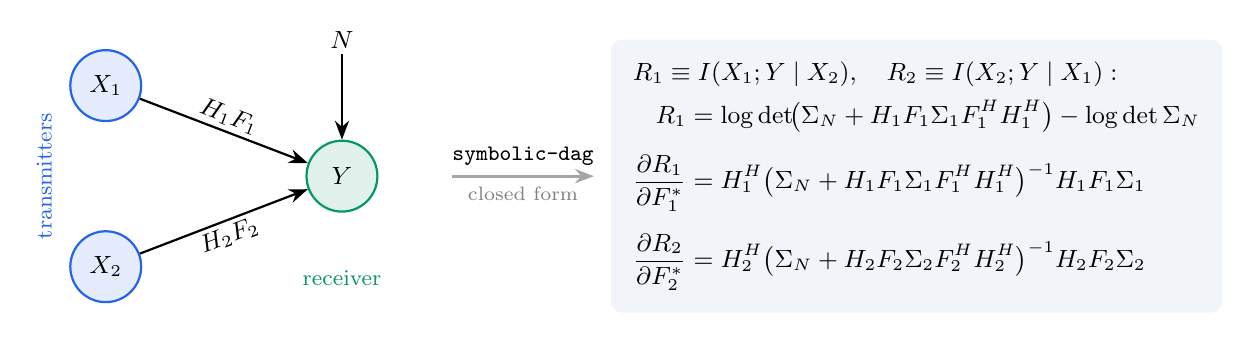
\begin{tikzpicture}[
  >={Stealth[length=2.4mm]}, thick, font=\small,
  node distance=10mm,
  src/.style={circle,draw=srccol,fill=srccol!12,minimum size=9mm,inner sep=0pt},
  rx/.style ={circle,draw=rxcol,fill=rxcol!12,minimum size=9mm,inner sep=0pt},
]
% --- the 2-user MIMO MAC (a linear Gaussian DAG) ---
\node[src] (x1) at (0,1.15) {$X_1$};
\node[src] (x2) at (0,-1.15) {$X_2$};
\node[rx]  (y)  at (3.0,0)   {$Y$};
\draw[->] (x1) -- node[above,sloped,inner sep=1.5pt]{$H_1 F_1$} (y);
\draw[->] (x2) -- node[below,sloped,inner sep=1.5pt]{$H_2 F_2$} (y);
% noise (a random variable) straight down into Y
\draw[->] (3.0,1.55) node[above,inner sep=1.5pt]{$N$} -- (y);
\node[below=6mm of y,rxcol,font=\footnotesize] {receiver};
% transmitters label, close to the two source nodes
\node[srccol,font=\footnotesize] at (-0.78,0) {\rotatebox{90}{transmitters}};

% --- the engine arrow ---
\draw[->,line width=1.1pt,gray!70] (4.4,0) -- (6.2,0)
  node[midway,above,black,font=\footnotesize\ttfamily]{symbolic-dag}
  node[midway,below,gray,font=\scriptsize]{closed form};

% --- the closed-form output (verbatim from the library, machine-verified) ---
\node[anchor=west,align=left,fill=boxcol,rounded corners=4pt,inner sep=8pt] at (6.4,0) {%
$\displaystyle R_1 \equiv I(X_1;Y\mid X_2),\quad R_2 \equiv I(X_2;Y\mid X_1):$ \\[4pt]
$\displaystyle
\begin{aligned}
R_1 &= \log\det\!\bigl(\Sigma_N + H_1 F_1 \Sigma_1 F_1\herm H_1\herm\bigr) - \log\det \Sigma_N \\[4pt]
\frac{\partial R_1}{\partial F_1^{*}} &= H_1\herm\bigl(\Sigma_N + H_1 F_1 \Sigma_1 F_1\herm H_1\herm\bigr)^{-1} H_1 F_1 \Sigma_1 \\[4pt]
\frac{\partial R_2}{\partial F_2^{*}} &= H_2\herm\bigl(\Sigma_N + H_2 F_2 \Sigma_2 F_2\herm H_2\herm\bigr)^{-1} H_2 F_2 \Sigma_2
\end{aligned}$};
\end{tikzpicture}
\end{document}
